\documentclass[11pt]{article}
\usepackage{hyperref}
\usepackage{graphicx} %m\'ethode pour ins\'erer des images version net
\DeclareGraphicsExtensions{.eps,.pdf,.png,.jpg,.JPG,.jpeg,.ps,.svg}

\usepackage{amsmath, verbatim}
\usepackage{amssymb}
\usepackage{fancyhdr}
\usepackage{pstricks}
\usepackage{pstricks-add}


\setlength{\oddsidemargin}{0.0in}
\setlength{\evensidemargin}{0.0in}
\setlength{\textheight}{8.4in}
\setlength{\textwidth}{6.5in}
\setlength{\voffset}{0.00in}
\setlength{\headsep}{26pt}
\setlength{\parindent}{0pt}
\setlength{\parskip}{6pt}

% header information
\pagestyle{fancyplain}
\lhead{MATH 150: Wednesday January 27}
\rhead{\textit{Spring Semester 2021}}



\chead{\textbf{Discussion 12: April 14th}}

\begin{document}
The goal of this discussion section is to get familiar with Markov chains.\\

Participation in discussion section counts as 5\% of the grade. Completion of the worksheets counts as 20\% of the grade. \textbf{Submit your worksheet work by {April 21st} at 2:59pm.}\\

Let's consider a model of population dynamics of two species in competition. We are interested to know which population will survive or if both might coexist after a long time. To model that we consider a finite birth and death chain $(X_n, Y_n)$ in $[0, \dots, n] \times [0, \dots, n] $  with the following transitions:
\begin{itemize}
\item $(i,j) \to (i,j)$ with a probability $m_{ij}$
\item $(i,j) \to (i+1,j)$ with a probability $p_{ij}$
\item $(i,j) \to (i,j+1)$ with a probability $q_{ij}$
\item $(i,j) \to (i-1,j)$ with a probability $r_{ij}$
\item $(i,j) \to (i,j-1)$ with a probability $s_{ij}$
\item $(0,0)$ is the only absorbing state (if you're at $(0,0)$ you remain there)
\item If one coordinate is $0$ or $n$, then there is no birth probability.
\end{itemize}
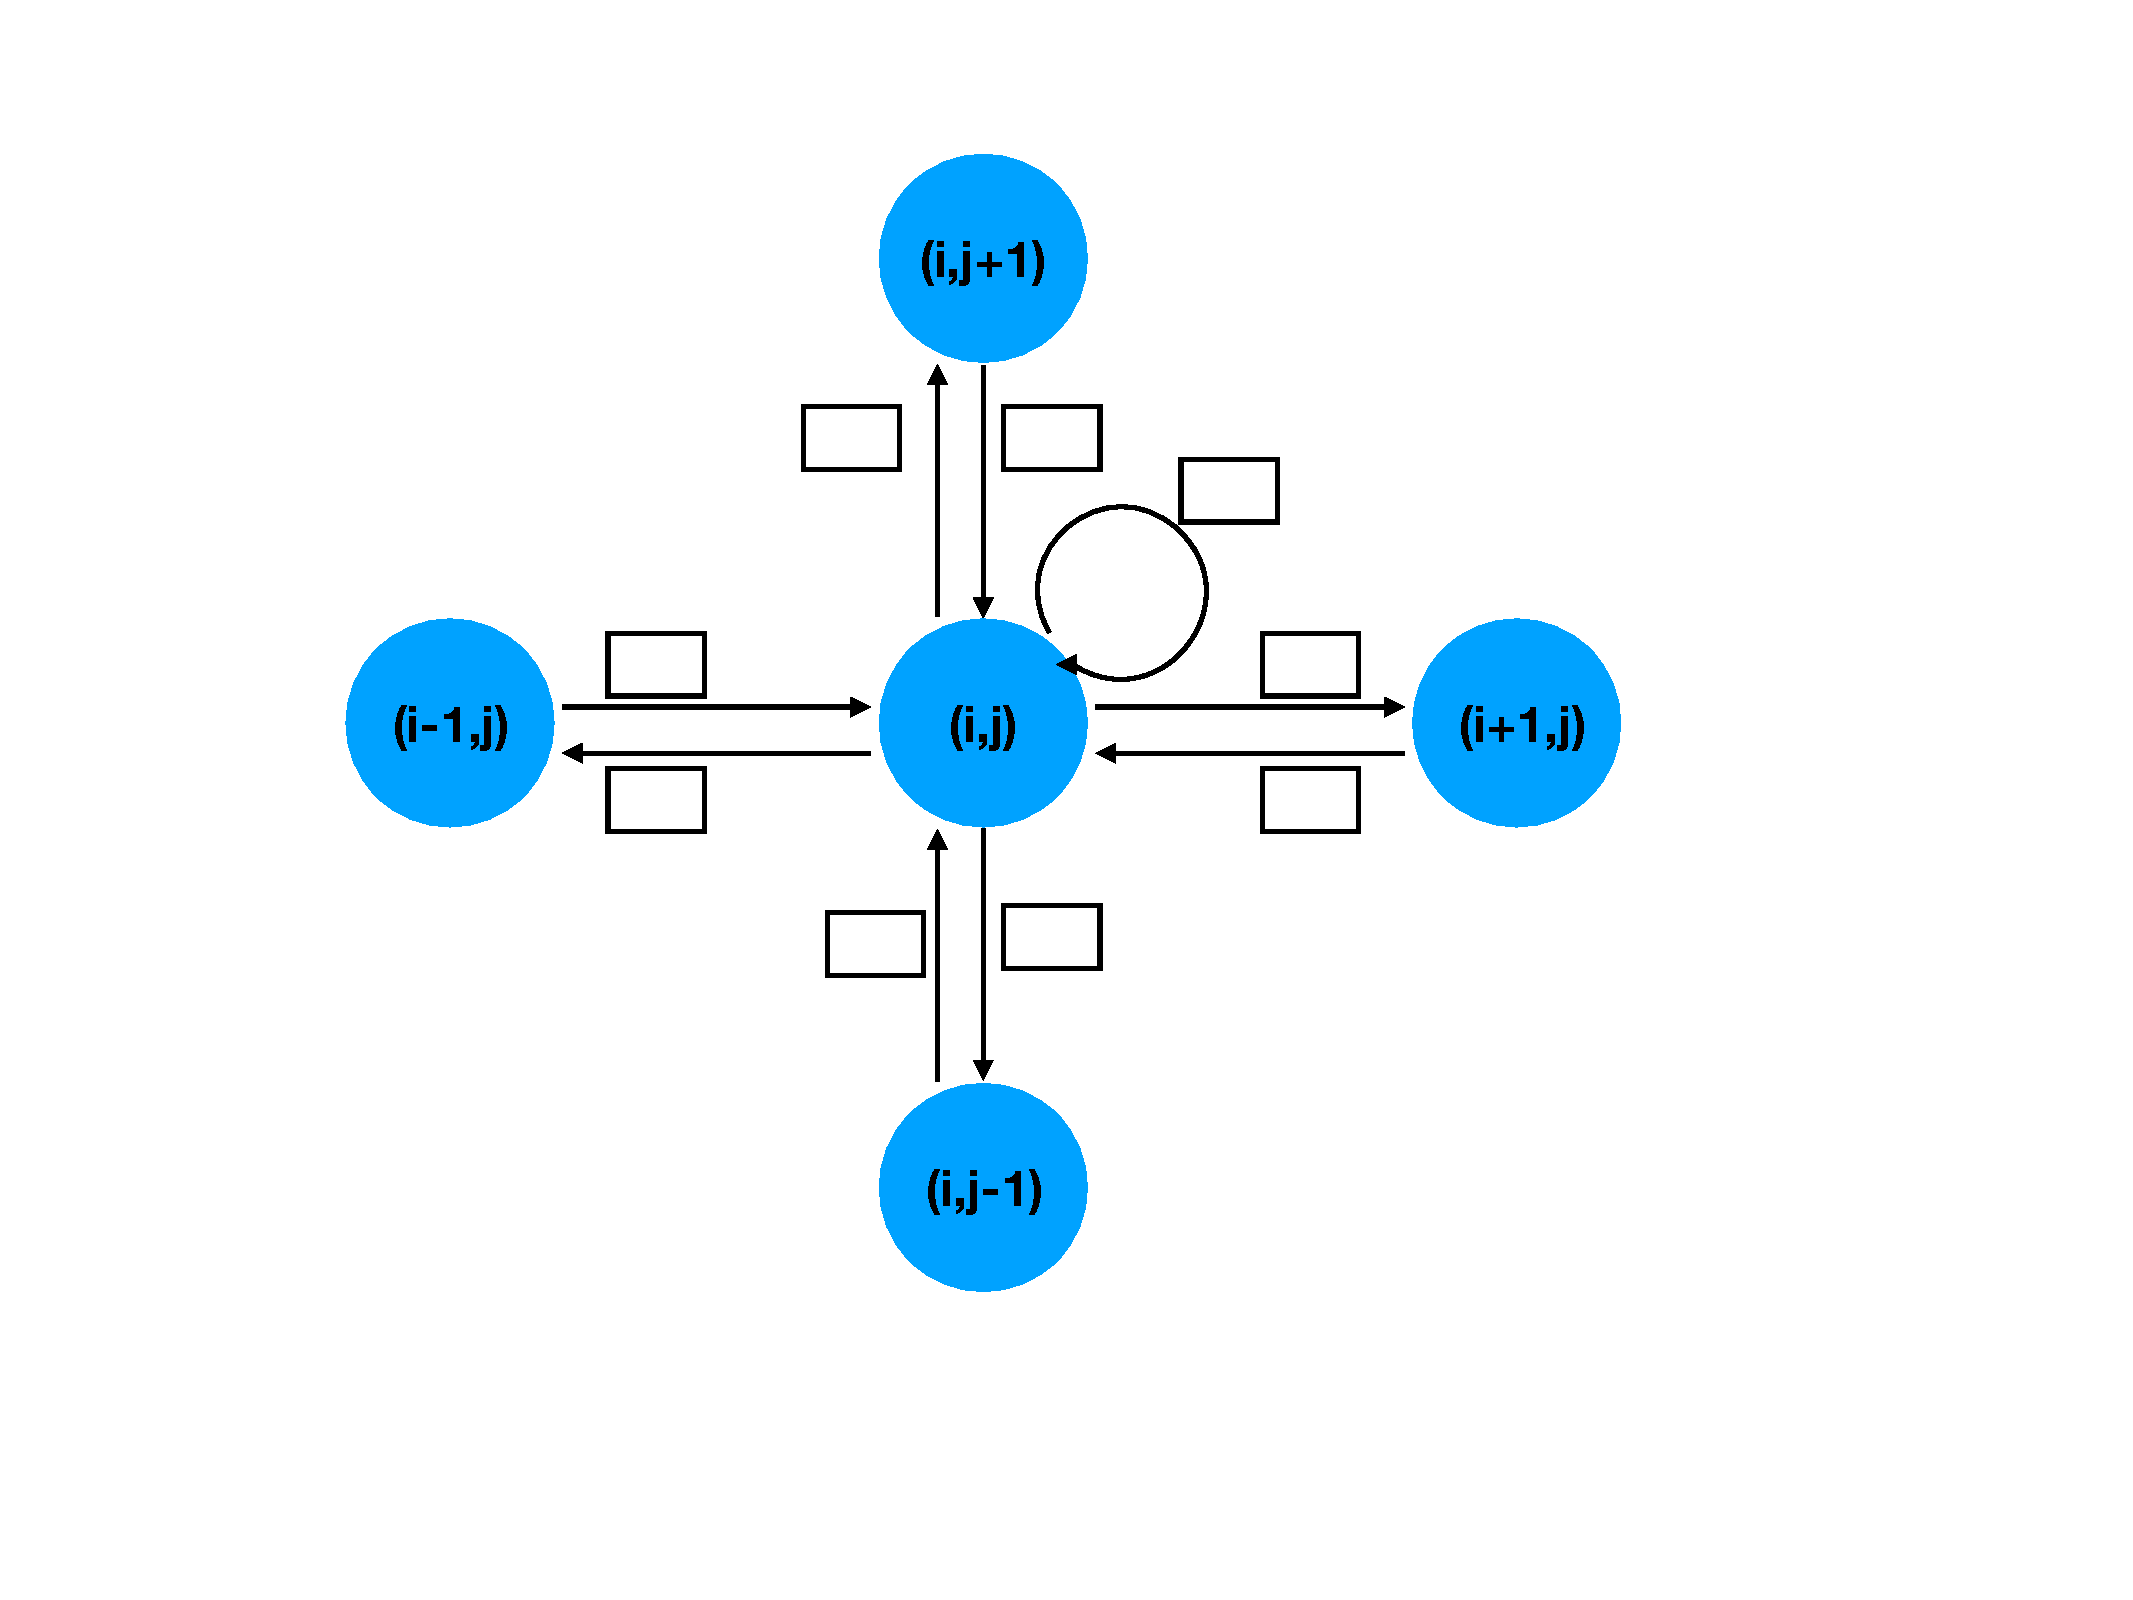
\includegraphics[width=0.5\linewidth]{fig1.pdf}
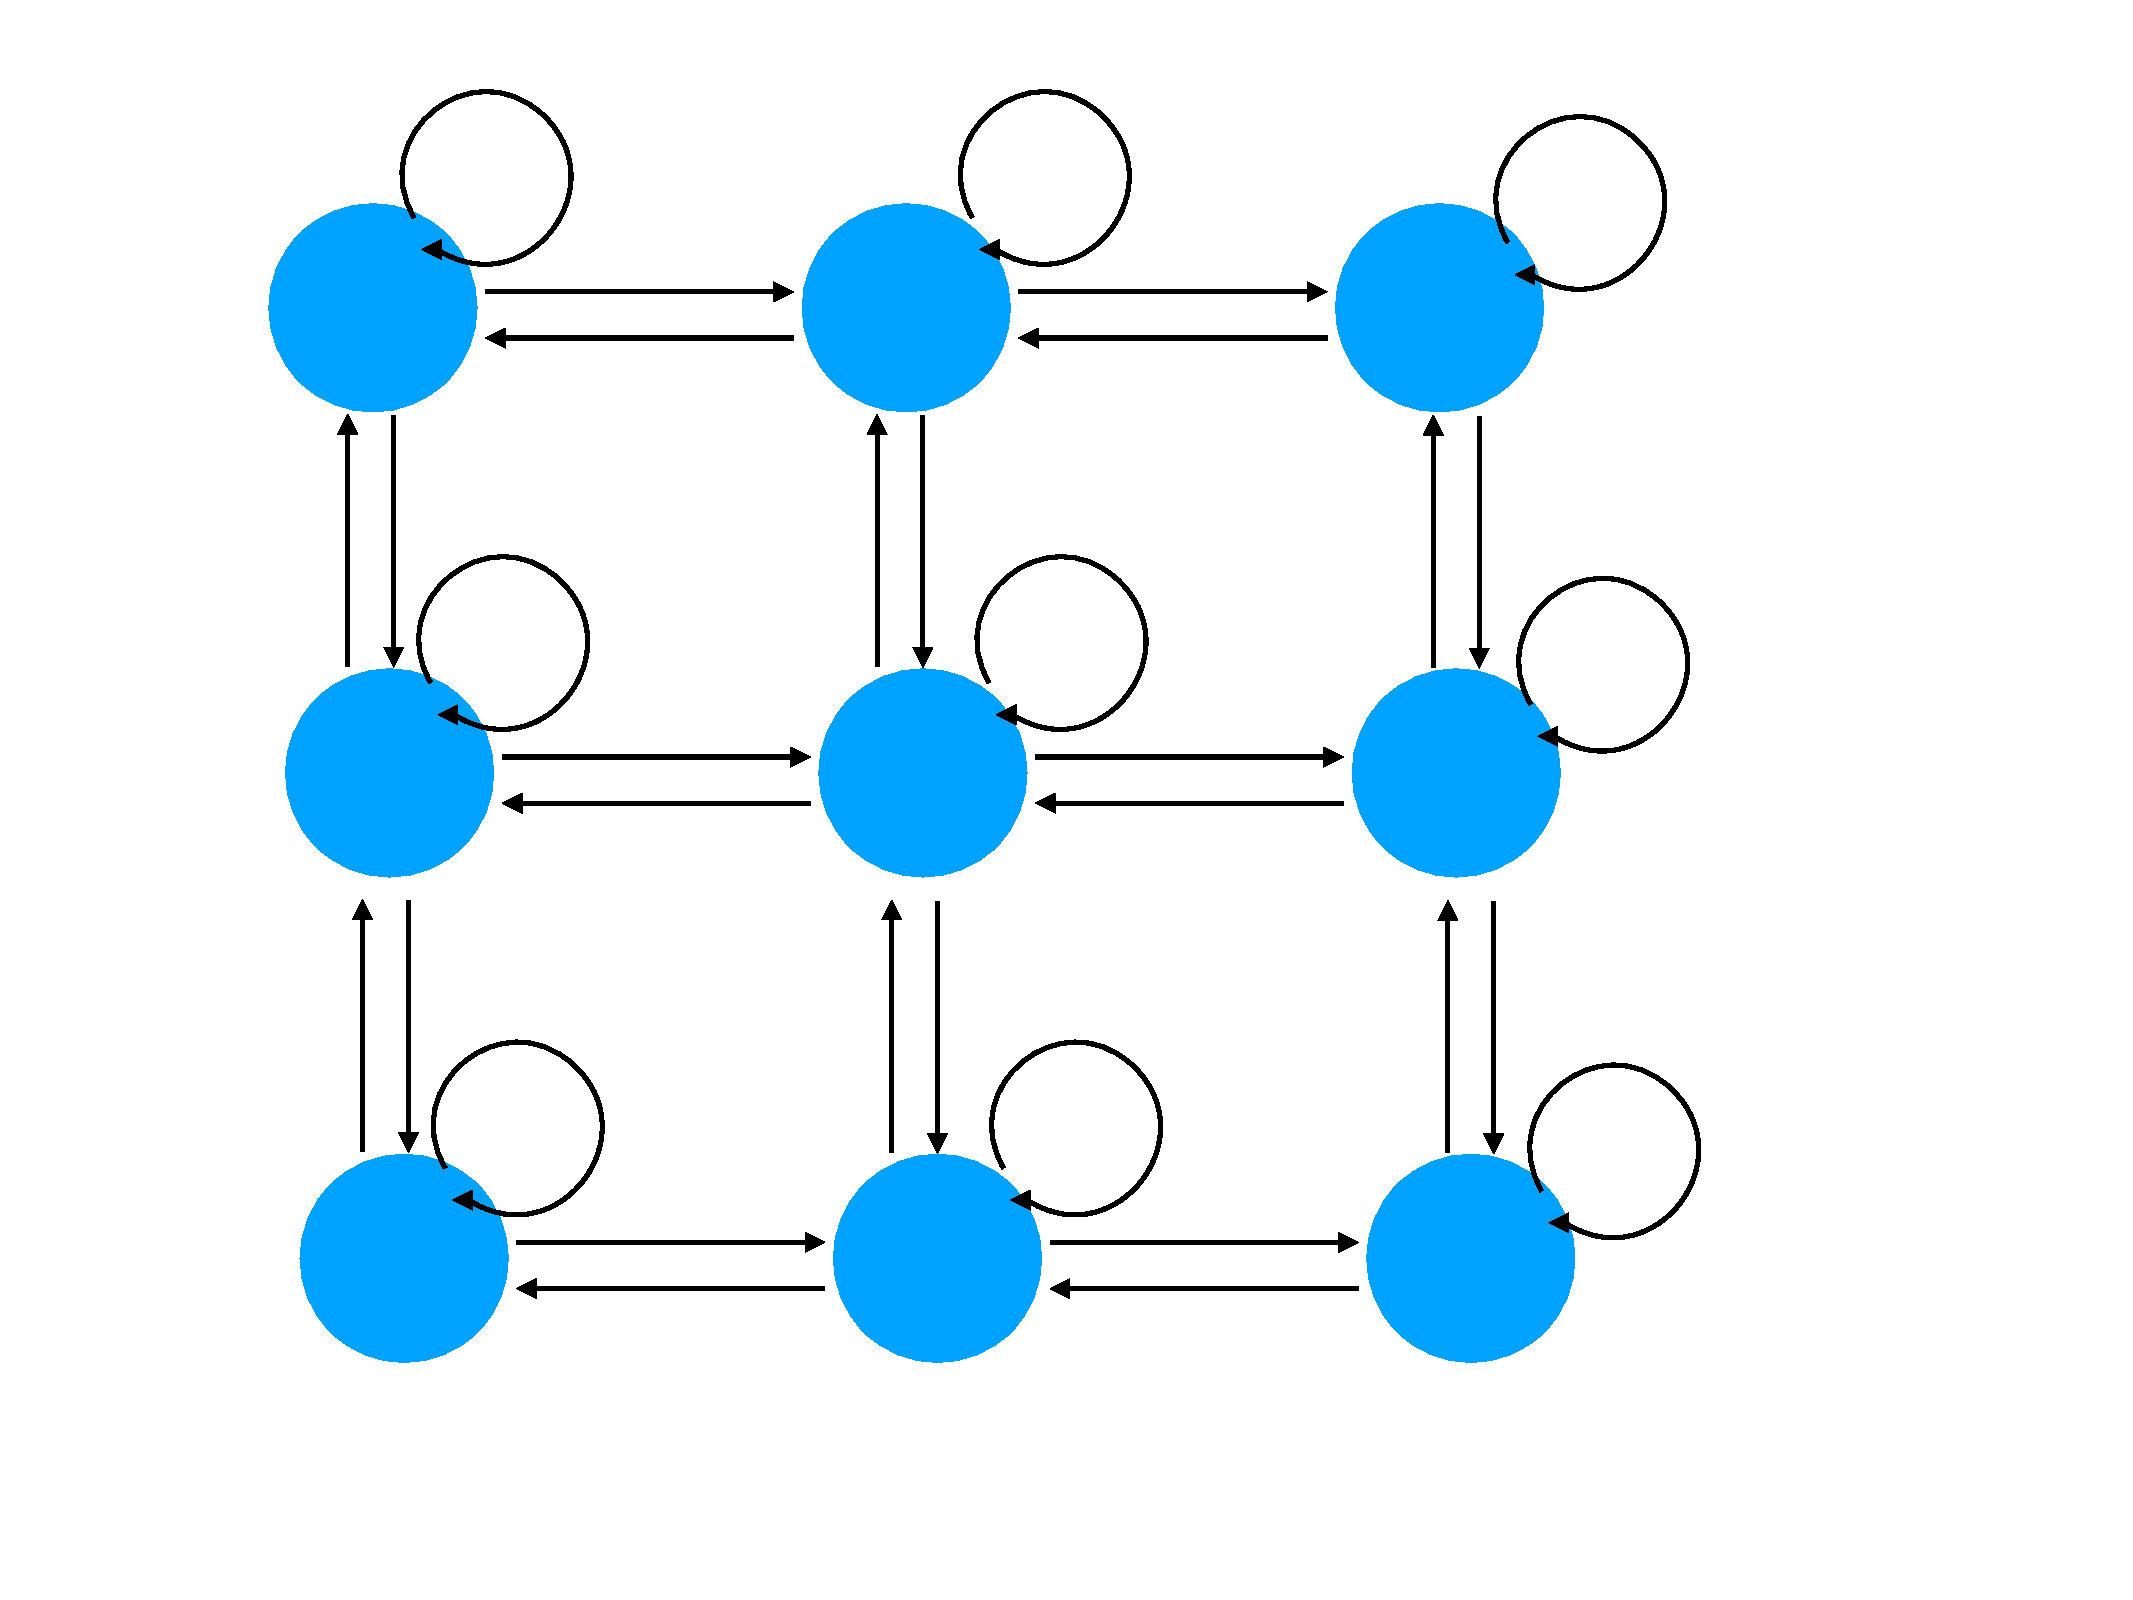
\includegraphics[width=0.5\linewidth]{fig2.pdf}
\begin{enumerate}
\item Complete the figure on the left.
\item For $n = 2$, try to sketch the associated Markov chain. Hint: define $A,B,C,D,E,F,G,H,I$ the 9 possible states using the figure on the right, and write the transition probability to go from one state to another.
\item Define the transition matrix $\mathcal{P}$.
\[\mathcal{P} = \underset{A\,\,\,\,\,\,B\,\,\,\,\,\,\,C\,\,\,\,\,\,\,D\,\,\,\,\,\,\,E\,\,\,\,\,\,\,F\,\,\,\,\,\,\,G\,\,\,\,\,\,\,H\,\,\,\,\,\,\,I}{\begin{pmatrix} ? &  ? &  ? &  ? &  ? &  ? &  ? &  ? &  ? \\
? &  ? &  ? &  ? &  ? &  ? &  ? &  ? &  ? \\
? &  ? &  ? &  ? &  ? &  ? &  ? &  ? &  ? \\
? &  ? &  ? &  ? &  ? &  ? &  ? &  ? &  ? \\
? &  ? &  ? &  ? &  ? &  ? &  ? &  ? &  ? \\
? &  ? &  ? &  ? &  ? &  ? &  ? &  ? &  ? \\
? &  ? &  ? &  ? &  ? &  ? &  ? &  ? &  ? \\
? &  ? &  ? &  ? &  ? &  ? &  ? &  ? &  ? \\
? &  ? &  ? &  ? &  ? &  ? &  ? &  ? &  ? \\
\end{pmatrix}} \begin{aligned} A \\ B \\ C \\ D \\ E \\ F \\ G \\ H \\ I \end{aligned}
\]
\item Using Python, assign some values for $m_{ij},p_{ij},q_{ij},r_{ij},s_{ij}$ (be consistent with the transition matrix properties) and predict the long-term distribution. Try for 3 different cases.
\item Submit your work on Catcourses under the assignment \texttt{Worksheet 12} \textbf{as a .ipynb}. 
\end{enumerate}

\end{document}
